
\section{Results \& Analysis}
\subsection{Testing Comparison}

As part of our analysis, we created the SSCTT Web-based User Interface, and we use it drastically streamline the pipeline for running Solidity contract test suites. And while it still currently only supports Oyente and Mythril, we've already been able make full-fledged security vetting of smart contracts possible for any person regardless of skill level. While it is not in the scope of this paper, we intend to perform a user study and formal evaluation of our tool in the future. Even without this, however, the impact of moving these test suites from command-line tools to fully managed and contained web-apps is clear. Users are able to see prettified results in order of importance to them. Furthermore, the accessibility benefit of automating the set-up and tear-down of the existing tools is motivated by the need for uneducated parties to be able to verify their smart contracts' security. Thus, we consider the Web Interface a success in this regard. \\

\subsection{Mutation Tests}

Both suites provide very different results when trying to analyze a Solidity script. To understand the reason behind this, we employed a combination of mutation testing and static analysis methods. On average, each script had 9.27 operations that were mutated to produce a list of mutated scripts. Then each of the two suites were run on the original Solidity files and on each of the mutations. \\

Figure \ref{tbl:Statistics} shows a summary of the errors and issues found by each suite across our collection of solidity scripts. Here we see that Oyente found 83\% more issues than Mythril on the original document, and 153\% more errors on the mutated scripts. On average SmartCheck found more bugs than Oyente in both cases, but a large part of this can be attributed to the scripts with no bugs. In these cases, Smart Check continues to detect bugs; thus leading to many false positives. With larger scripts with many bugs, Oyente and Mythril significantly detect more bugs than SmartCheck. However, in general smart contracts are usually smaller, and define a very specific purpose of ensuring transactions are completed according to all parties. \\

\subsection{Static Analysis}

To study the suites in more detail, we plotted the number of bugs found by each suite (Figure \ref{bugs} Left, Middle). If each suite were exactly the same, then each point would lie on the $y=x$ line. However, in the first plot we see a consistent trend to the right of this line. This means that Oyente has found more bugs in every script than Mythril. For the middle plot, we perform the same comparison of Oyente and Smartcheck. For this comparison, we see a sections of tests where SmartCheck finds more bugs, and another section where Oyente does. On further inspection, SmartCheck finds more bugs on the smaller less buggy scripts; while Oyente is significantly better at detecting bugs in the larger more complicated scripts.  This trend is minimally impacted by mutations in the code, but for the Oyente vs. Mythril comparison it is clear that that Oyente outperforms Mythril on mutated scripts.\\

The plot to the right of Figure \ref{bugs} shows the number of bugs as a function of complexity of the script. Here we see a trend where scripts that are smaller and scripts that are larger tend to have more bugs. It is expected that a larger script would have more bugs, but scripts with average complexity have much less bugs than low complexity scripts.  SmartCheck breaks this trend by having many more bugs with the smaller scripts, and less with the larger scripts. A possible explanation for this is that smaller scripts tended to have significantly less error handling; thus bugs would be caught less. Moreover, SmartCheck tends to focus on bad error handling where the other suites ignore this altogether.  \\

\subsection{Specific Bugs}

Although quantity of bugs is important, specific bugs are responsible for the DAO attack and can cause insecurities in the contracts. Thus, focusing on the quality of the bugs is vital for smart contract testing suites. Specifically, we tested a smart contract that checks if a given any address is valid. For this contract, Oyente detects a possible integer underflow, SmartCheck states that one of the variables in the function could be private but was defined as public (\texttt{SOLIDITY\_VISIBILITY}), and Mythril provides a meaningful warning that having no validation on the input address allows for users to provide injection attacks using this function. For both Oyente and SmartCheck, their bugs offer no security vulnerabilities or possible solutions, while Mythril describes the specific threat and why it is a threat.  

Like previously mentioned, some of the vulnerabilities that we found were of high quality and very notable in the sense that they have previously been exploited to in famous hacks. For example, Mythril error-checks a contract by looking for inputs that trigger and unprotected SUICIDE or SELFDESTRUCT instruction. With this instruction, a smart contract is essentially destroyed and all the remaining balance of the contract to a specified address. This bug was famously revealed in November 2017, when an anonymous Github user "accidentally" became the owner of the main library contract and then proceeded to self-destruct it. Because he was successfully able to call an unprotected self-destruct instruction, about \$300 million was frozen and inaccessible forever. Presumably, had this contract been debugged using the Mythril test suite, this error would have been caught.  

Another such example comes from the highly publicized DAO attack. In the DAO attack, a hacker made use of a "reentrancy" bug to drain Ethereum from the DAO. Reentrancy attacks occur when the external contract called by the initial contract is allowed to make new calls to the calling contract before the initial execution is complete. In this way, an untrustworthy external contract can take advantage of the callee contract. Oyente looks for such reentrancy issues in contracts, once again showing the quality of the vulnerabilities we found. 

Furthermore, these findings also justify the need for our tool. Since Oyente, Mythril, and SmartCheck are implemented differently, they look for different types of issues. Therefore, to get the best coverage on your code, the use of multiple tools is highly encouraged. However, all of these tools run on different environment and are hard to find unless one is to search for them by name. Our tool is also easy to update - a test suite can easily be added. Therefore, we provide a useful, simple platform for a developer to take advantage of all the tools available to them.   

\begin{figure*}[h!]
\centering
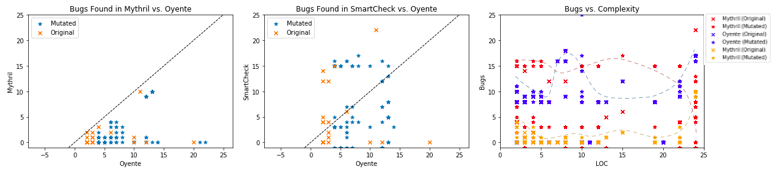
\includegraphics[width=7.0in]{img/Bugs2.png}
\caption{Plots of the number of bugs found with each suite (Left, Middle) and the number of bugs found as a function of the script's complexity (Right). Here we see that Oyente consistently detects more bugs than Mythril, but SmartCheck detects the most bugs of all suites. Moreover, the number of bugs does not increase monotonically in complexity, but is bimodal where lowest and highest complexity lead to more bugs.}
\label{bugs}
\end{figure*}

